\documentclass{article}
\author{}

\usepackage{graphicx}
\usepackage{wrapfig}
\usepackage{enumerate}
\usepackage{hyperref}
\usepackage{float}
\usepackage[margin = 2.25cm]{geometry}
\usepackage[table]{xcolor}
\usepackage{fancyhdr}
\hypersetup{
  colorlinks = true,
  urlcolor = blue
}
\setlength\parindent{0pt}
\pagestyle{fancy}
\fancyhf{}
\rhead{College of Engineering, Construction and Living Sciences\\Bachelor of Information Technology}
\lfoot{Practical 14 Django 8: Django REST Framework \\Version 1, 2020}
\rfoot{\thepage}

\begin{document}

\begin{figure}
	\centering
	
\includegraphics[width=50mm]{./img/logo.png}
\end{figure}

\title{College of Engineering, Construction and Living Sciences\\Bachelor of Information Technology\\IN608: Intermediate Application Development Concepts\\Level 6, Credits 15\\\textbf{Practical 14 Django 8: Django REST Framework}} 
\date{}
\maketitle

\textbf{Due Date:} 14/09/2020 at 5pm \\

In this practical, you will complete a series of tasks covering today's lecture. This practical is worth 1\% of the final mark for the IN608: Intermediate Application Development Concepts course. \\

Before you start, in your practicals repository, create a new branch called \textbf{14-practical}.

\section*{Task} 
Create a Django project called \texttt{quizcreatordrf}. \texttt{cd} to \texttt{quizcreatordrf}, create a virtual environment \& install Django. Create an app called \texttt{practical14quizcreatordrf}. Please ensure you configure your app in \texttt{quizcreatordrf/settings.py} \& \texttt{quizcreatordrf/urls.py}. \\

In order to create a Django REST API, the \texttt{djangorestframework} Python module must be installed. Run the command \texttt{pipenv install djangorestframework} to install the \texttt{djangorestframework} Python module. In \texttt{settings.py}, declare \texttt{rest\_framework} in \texttt{INSTALLED\_APPS}. \\

In the \texttt{models.py}, copy \& paste the \texttt{User} \& \texttt{Quiz} model from \textbf{Practical 12 Django 6: Authentication}. \\

Create two files called \texttt{serializer.py} \& \texttt{urls.py}. In \texttt{serializer.py}, create two classes called \texttt{UserSerializer} \& \texttt{QuizSerializer} which implement \texttt{serializers.ModelSerializer}. For each class, create a nested class called \texttt{Meta}. In the \texttt{Meta} class, declare the appropriate \texttt{model} \& \texttt{fields}. \\

In \texttt{view.py}, create two classes called \texttt{UserViewSet} which implements \texttt{viewsets.ReadOnlyModelViewSet} \& \texttt{QuizViewSet} which implements \texttt{viewsets.ModelViewSet}. For each class, declare the appropriate \texttt{queryset} \& \texttt{serializer\_class}, i.e., \texttt{User.objects.all()} \& \texttt{UserSerializer}. \\

In \texttt{urls.py}, create two URLs which map to \texttt{UserViewSet} \& \texttt{QuizViewSet}. The URL patterns should be as follows:
\begin{itemize}
  \item api/user
  \item api/quiz
\end{itemize} 

In \texttt{settings.py}, set permission policy so that the API is restricted to \texttt{only} admin users.

\subsection*{Expected Output} 
Run the command \texttt{python manage.py runserver} then navigate to \href{http://127.0.0.1:8000/practical14quizcreatordrf/api}{http://127.0.0.1:8000/practical14quizcreatordrf/api} \\

\begin{figure}[H]
  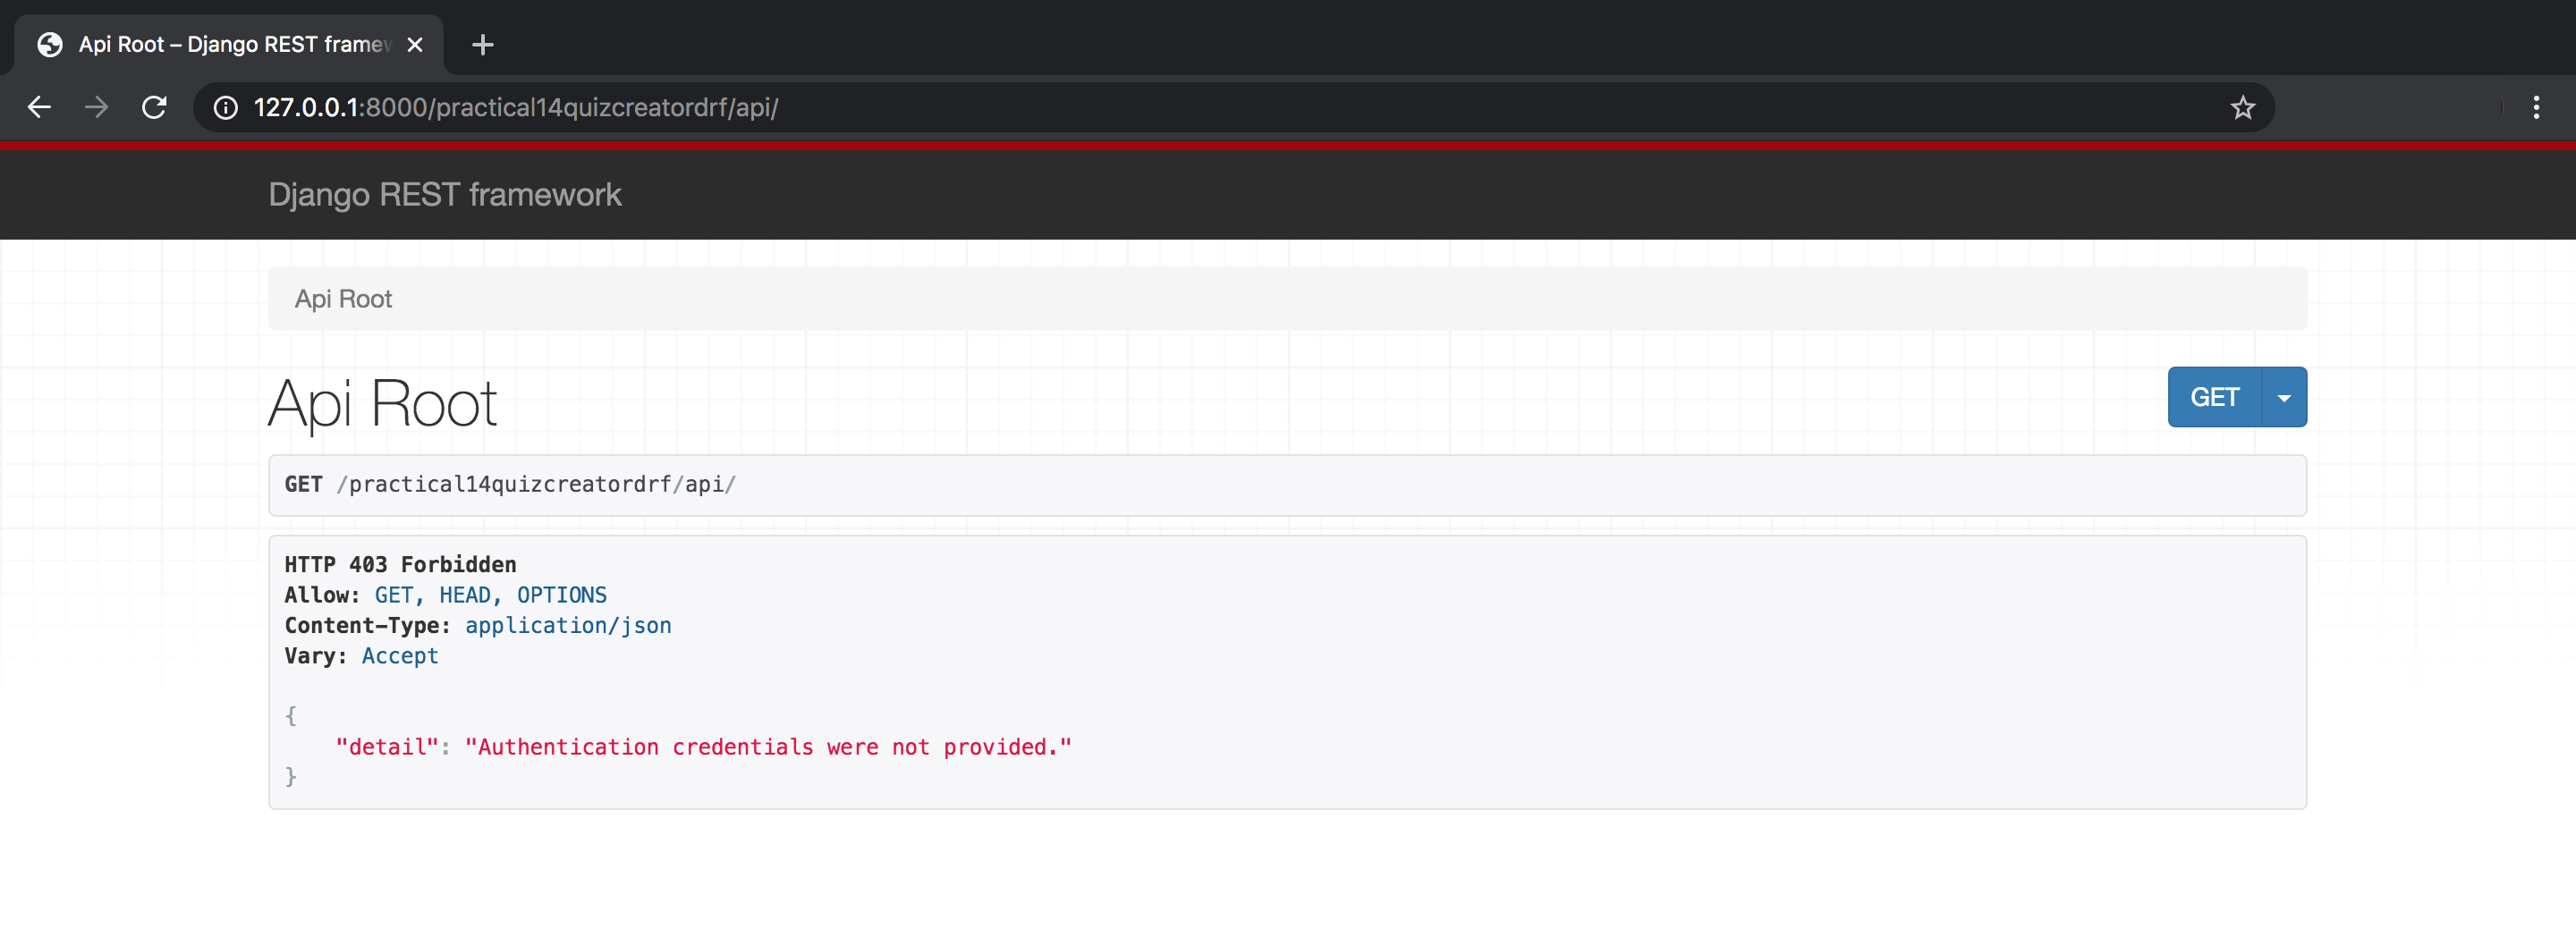
\includegraphics[width=175mm, height=65mm]{./img/14-expected-drf-1.png}
  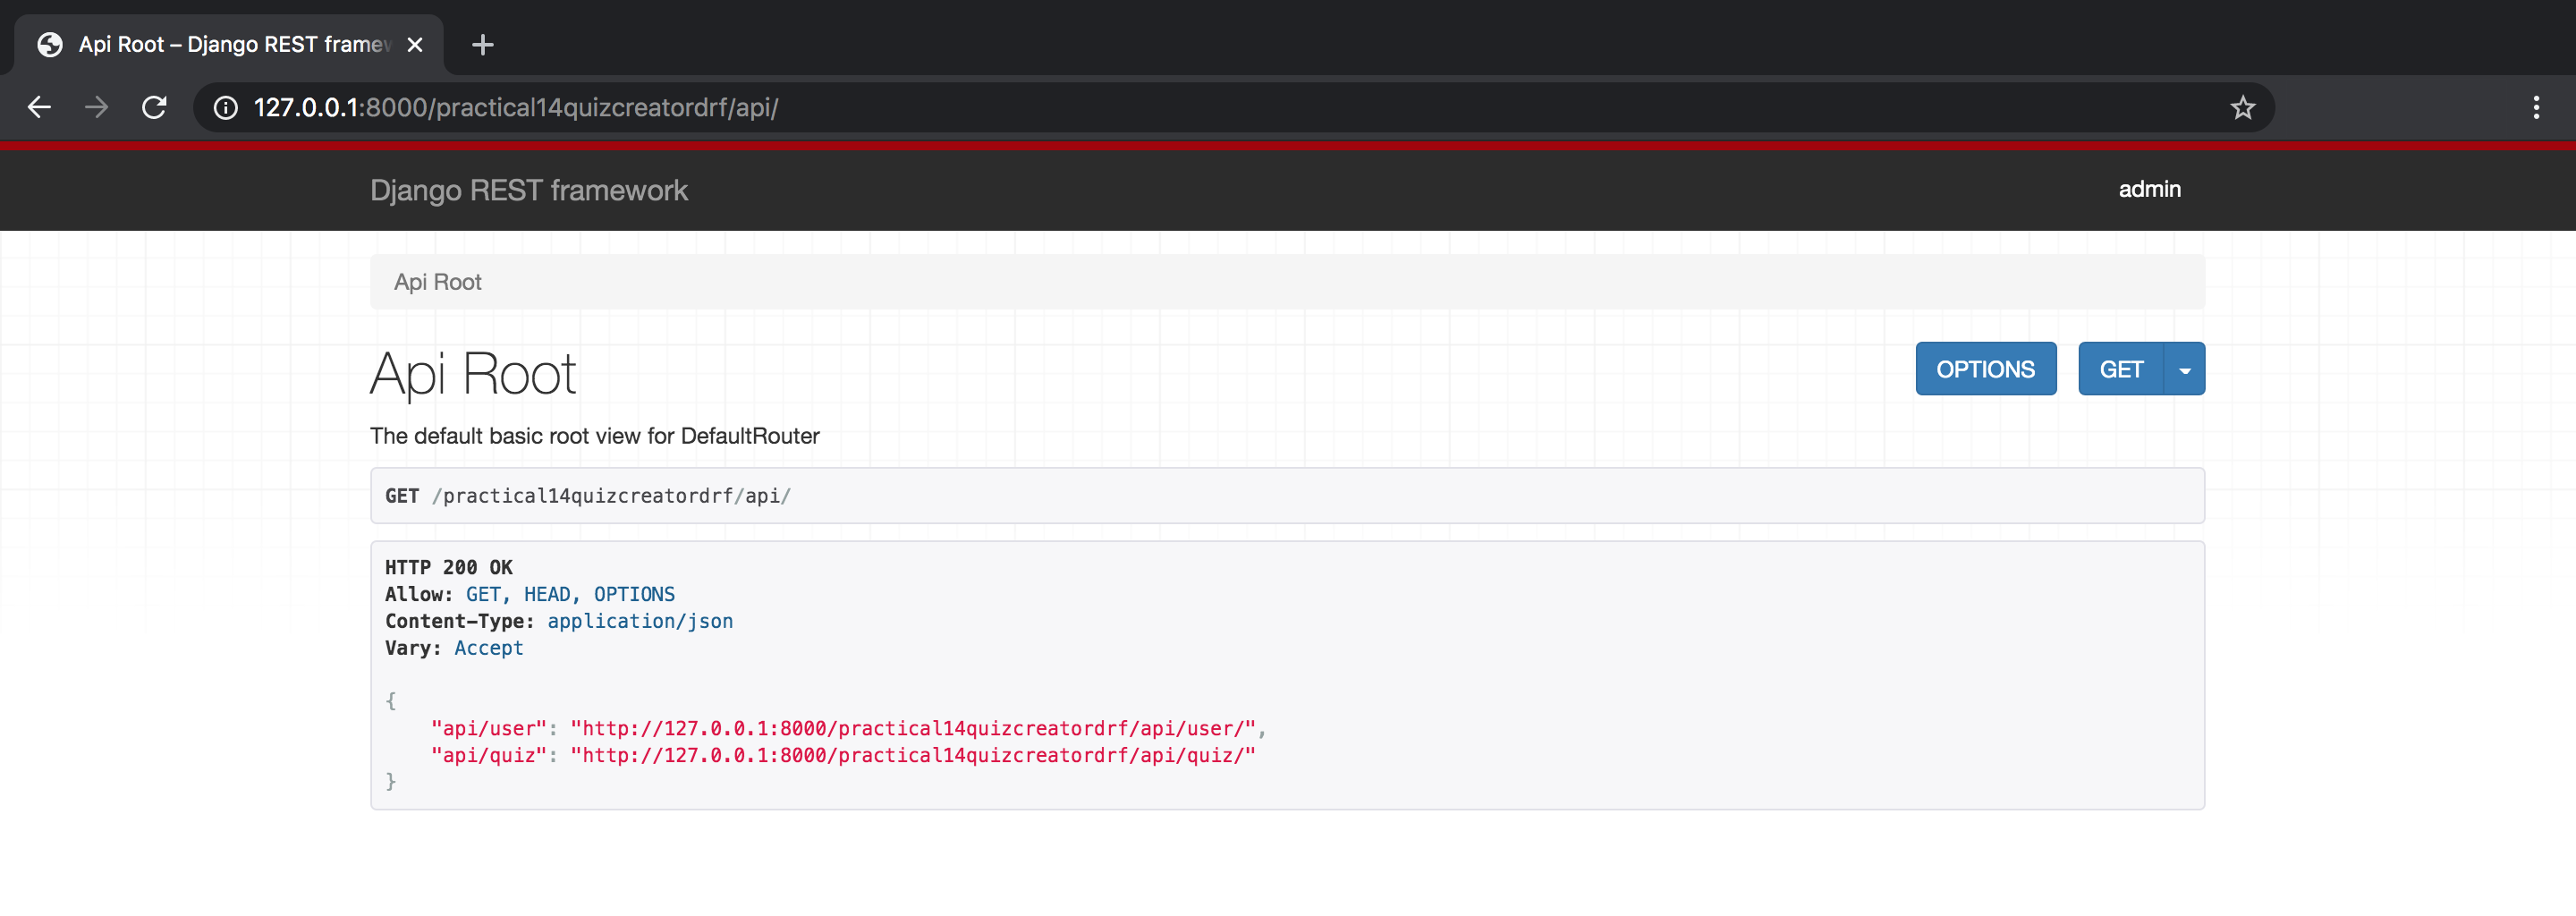
\includegraphics[width=175mm, height=65mm]{./img/14-expected-drf-2.png}
\end{figure}

\begin{figure}[H]
  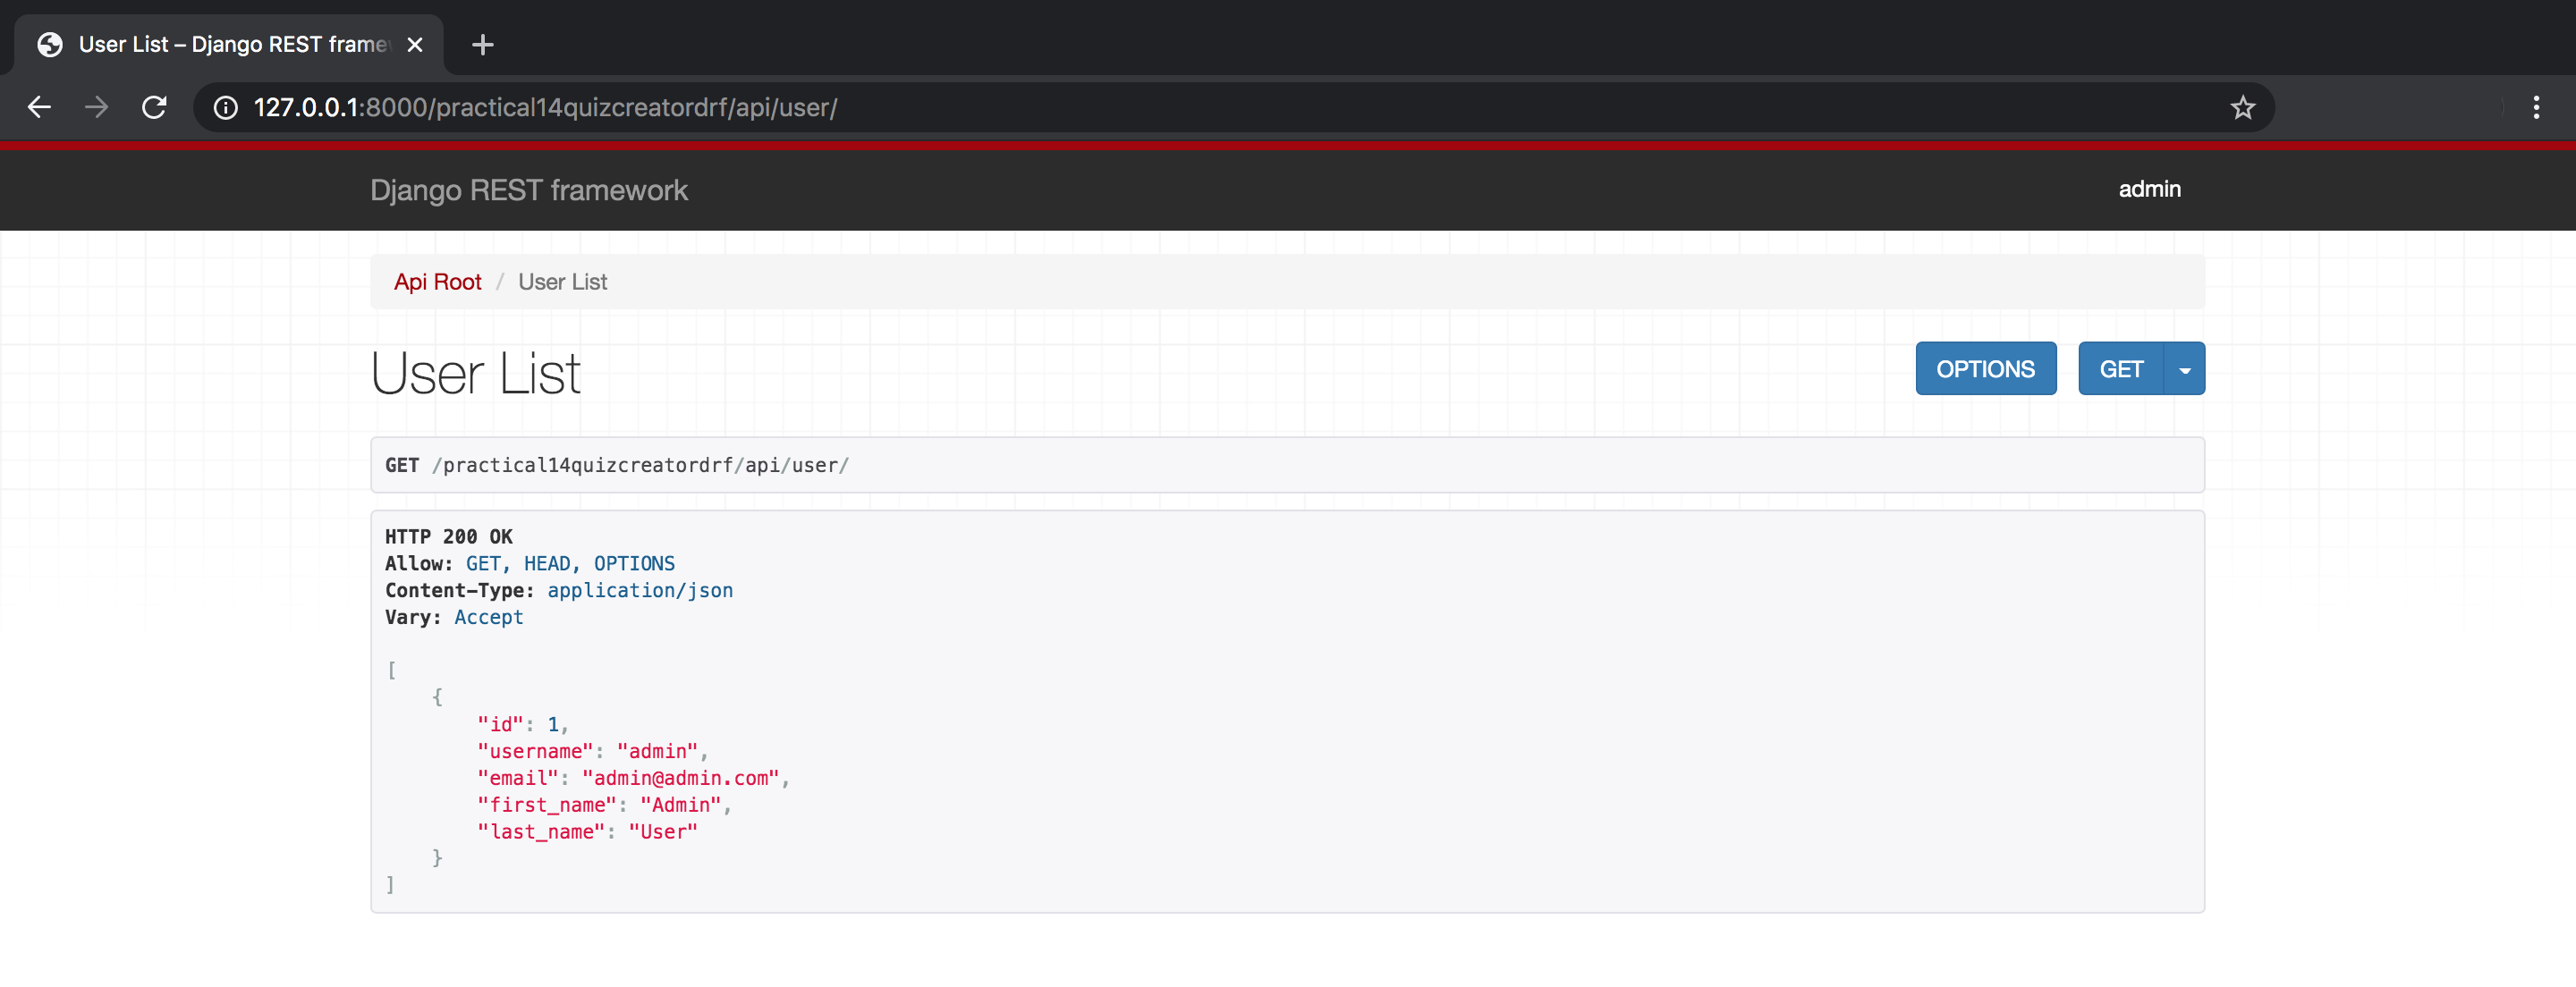
\includegraphics[width=175mm, height=65mm]{./img/14-expected-drf-3.png}
  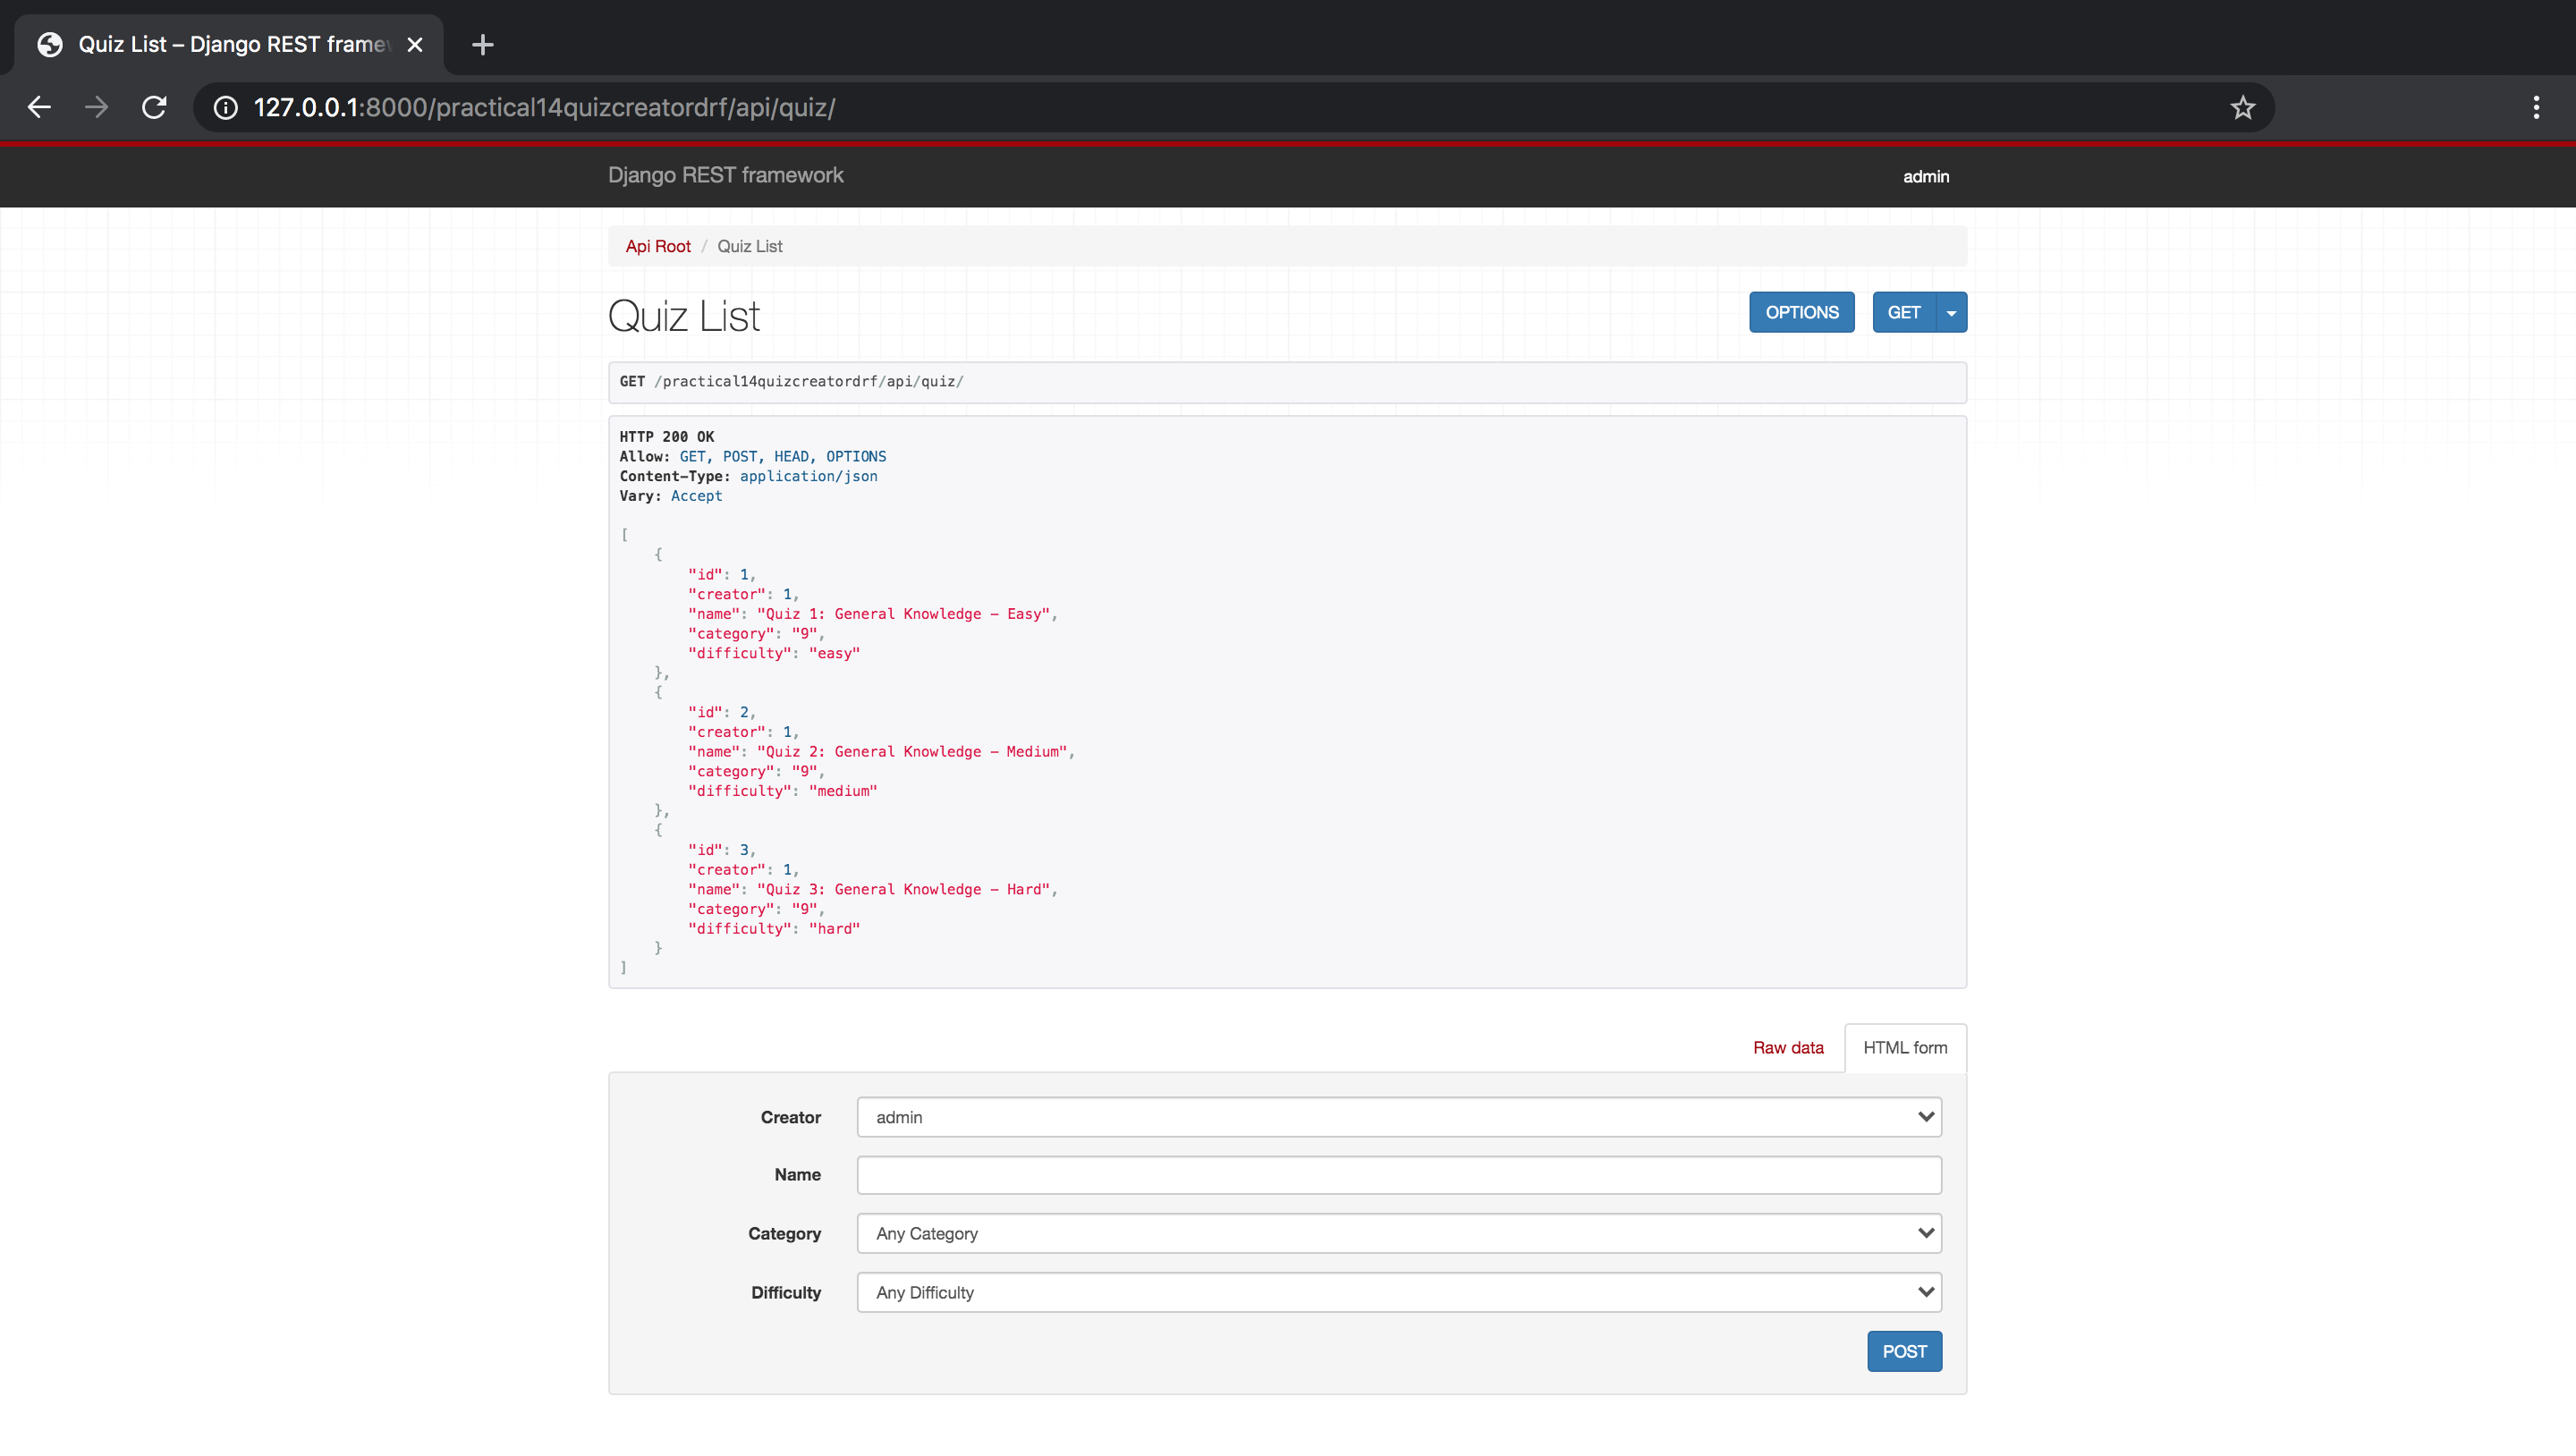
\includegraphics[width=175mm, height=95mm]{./img/14-expected-drf-4.png}
\end{figure}

\begin{figure}[H]
  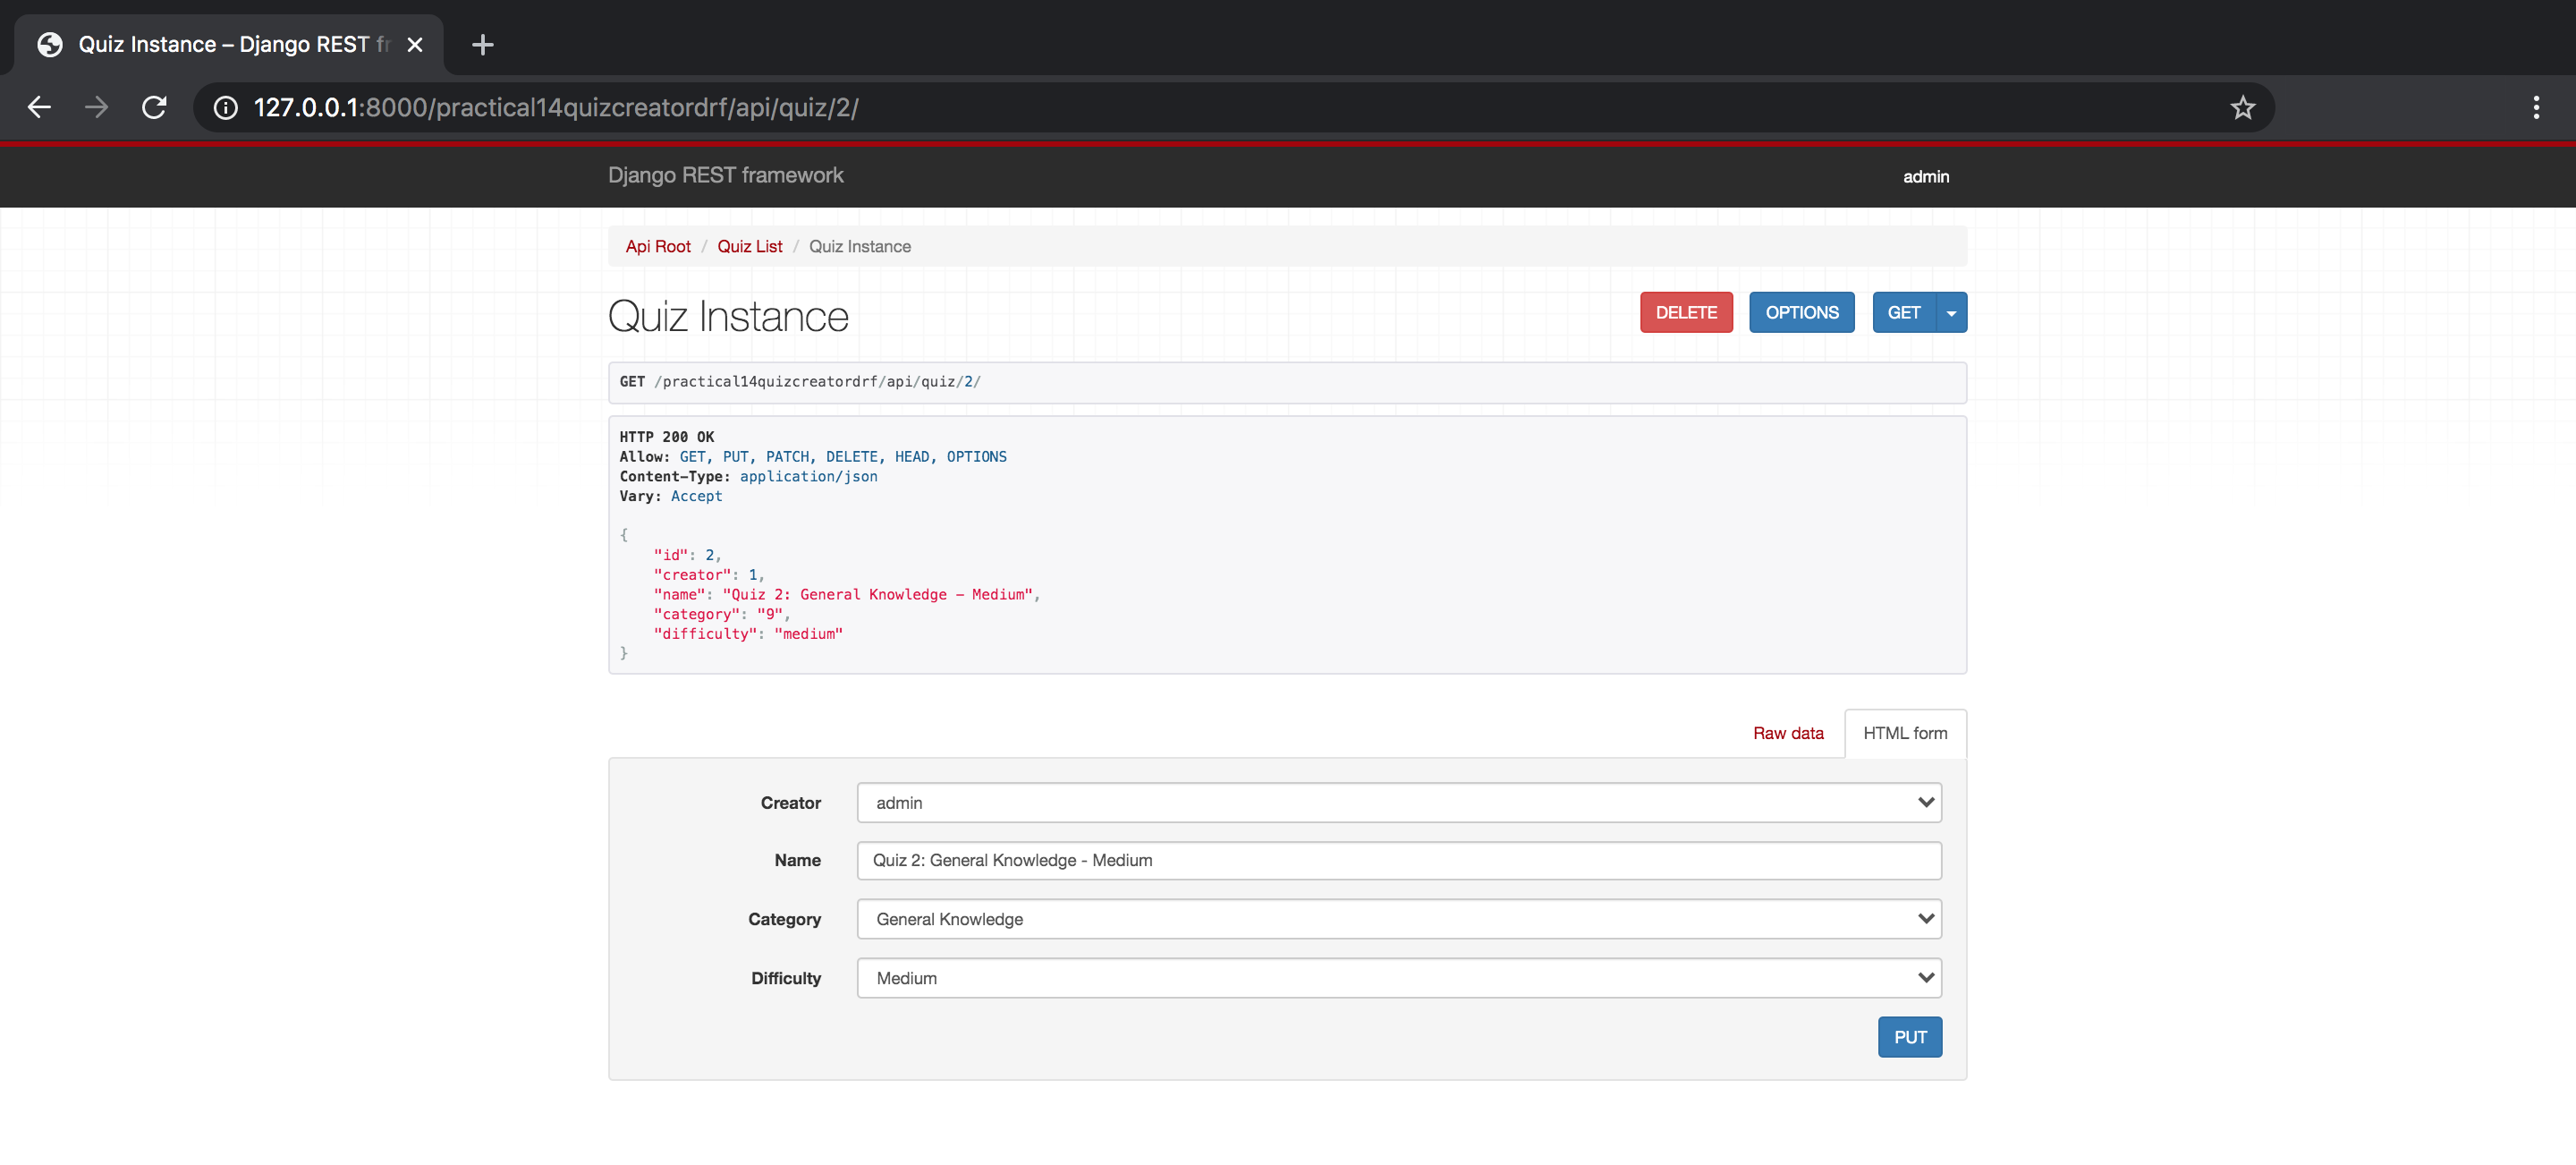
\includegraphics[width=175mm, height=90mm]{./img/14-expected-drf-5.png}
\end{figure}

\textbf{Deployment link:} \href{https://int-app-dev-practical-14.herokuapp.com/practical14quizcreatordrf/api}{https://int-app-dev-practical-14.herokuapp.com/practical14quizcreatordrf/api}

\subsection*{Resources} 
\begin{itemize}
  \item \href{https://www.django-rest-framework.org/}{Django REST Framework}
\end{itemize}

\end{document}